\begin{figure}
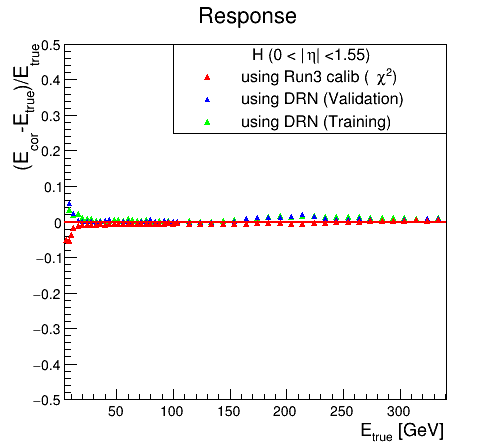
\includegraphics[width=0.495\textwidth]{./plots_pdf/HCAL_plots/Trained_target_ratioflip_0_500_10/pdf/H_barrel/barrel_corrEtaBarrelHcal.png}
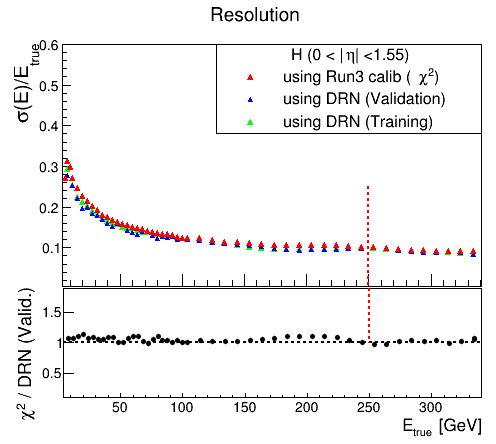
\includegraphics[width=0.495\textwidth]{./plots_pdf/HCAL_plots/Trained_target_ratioflip_0_500_10/pdf/H_barrel/barrel_corrEtaBarrelHcal_reso.png}

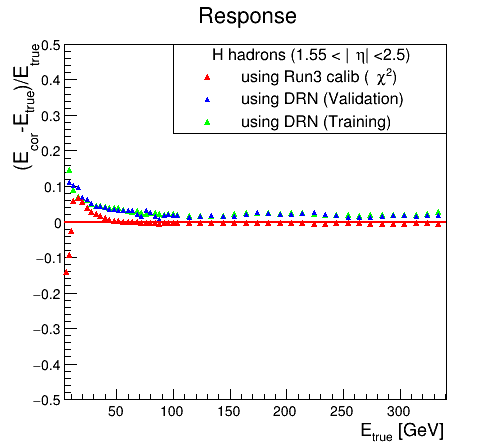
\includegraphics[width=0.495\textwidth]{./plots_pdf/HCAL_plots/Trained_target_ratioflip_0_500_10/pdf/H_ec_in/EC_within_tracker_corrEtaEndcapHcal.png}
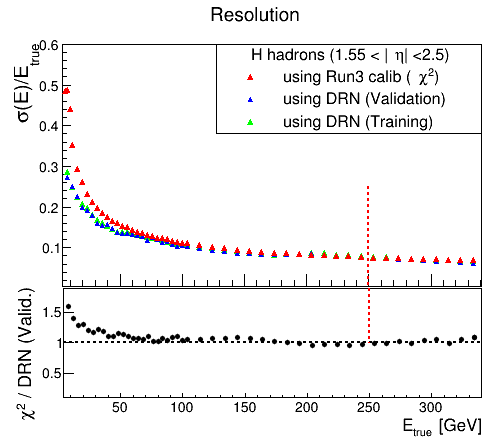
\includegraphics[width=0.495\textwidth]{./plots_pdf/HCAL_plots/Trained_target_ratioflip_0_500_10/pdf/H_ec_in/EC_within_tracker_corrEtaEndcapHcal_reso.png}

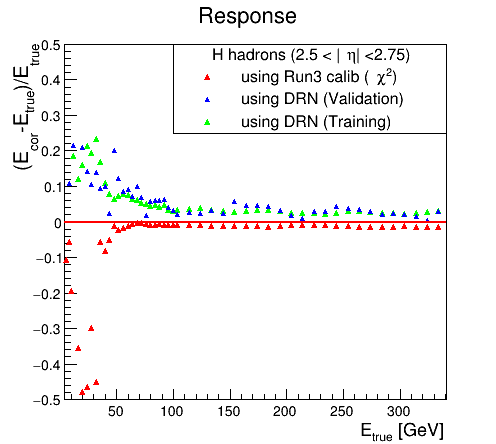
\includegraphics[width=0.495\textwidth]{./plots_pdf/HCAL_plots/Trained_target_ratioflip_0_500_10/pdf/H_ec_out/EC_outside_tracker_corrEtaEndcapHcal.png}
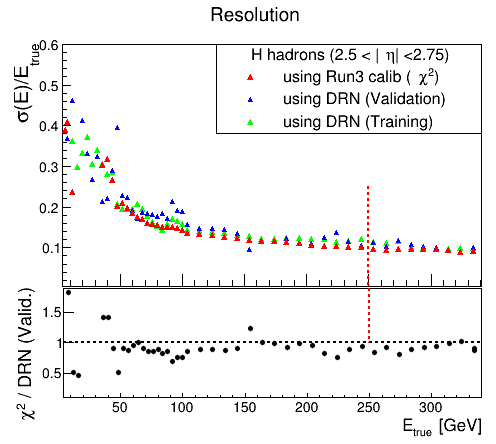
\includegraphics[width=0.495\textwidth]{./plots_pdf/HCAL_plots/Trained_target_ratioflip_0_500_10/pdf/H_ec_out/EC_outside_tracker_corrEtaEndcapHcal_reso.png}
\caption[Response (resolution) vs. \pt of the PF H-hadron cluster - traget trueE]{Mean response (resolution) defined by calibrated PF EH-hadron clusters using $\chi^{2}$ method (red), DRN model derived from training samples (green), DRN model validated on testing samples (blue). (top) barrel, (middle) endcap within the tracker, and (bottom) endcap outside the tracker. DRN training target is trueE.}
\label{fig:H_trueE}
\end{figure}
